\begin{comment}
\[
    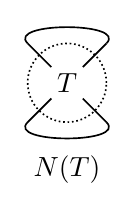
\begin{tikzpicture}[baseline=-0.65ex, scale=0.1]
    \useasboundingbox (-5, -11) rectangle (5, 7);
        \draw[semithick] (-2, -2) to (-5,-5);
        \draw[semithick] (2, 2) to (5,5);
        \draw[semithick] (2, -2) to (5,-5);
        \draw[semithick] (-2, 2) to (-5,5);        %
        \draw[semithick, densely dotted] (-0, 0) circle (5);
        \node at (0, 0) {$T$};
        \node [below] at (0, -8) {$N(T)$};
        \draw[semithick] (-5, -5) [in=-45, out=-135] to (5, -5);        %
        \draw[semithick] (-5,    5) [in=45, out=135] to (5, 5);        %
    \end{tikzpicture}
    \quad \quad
    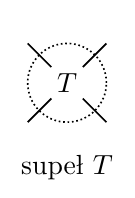
\begin{tikzpicture}[baseline=-0.65ex, scale=0.1]
    \useasboundingbox (-5, -11) rectangle (5, 7);
        \draw[semithick] (-2, -2) to (-5,-5);
        \draw[semithick] (2, 2) to (5,5);
        \draw[semithick] (2, -2) to (5,-5);
        \draw[semithick] (-2, 2) to (-5,5);        %
        \draw[semithick, densely dotted] (-0, 0) circle (5);
        \node at (0, 0) {$T$};
        \node [below] at (0, -8) {supeł $T$};
    \end{tikzpicture}
    \quad \quad
    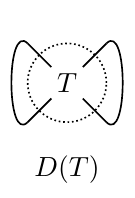
\begin{tikzpicture}[baseline=-0.65ex, scale=0.1]
    \useasboundingbox (-5, -11) rectangle (5, 7);
        \draw[semithick] (-2, -2) to (-5,-5);
        \draw[semithick] (2, 2) to (5,5);
        \draw[semithick] (2, -2) to (5,-5);
        \draw[semithick] (-2, 2) to (-5,5);        %
        \draw[semithick, densely dotted] (-0, 0) circle (5);
        \node at (0, 0) {$T$};
        \node [below] at (0, -8) {$D(T)$};
        \draw[semithick] (-5, -5) [in=135, out=-135] to (-5, 5);        %
        \draw[semithick] (5, -5) [in=45, out=-45] to (5, 5);        %
    \end{tikzpicture}
    \quad \quad
\]
\end{comment}